\documentclass[12pt]{article} 

\usepackage[utf8]{inputenc}
\usepackage[OT1]{fontenc}

% Gestion de la langue du document
\usepackage[french]{babel}

% Gestion des espaces
\usepackage{xspace}

% Gestion des images
\usepackage{graphicx}

% Pour permettre la redéfinition des dimensions
\usepackage[a4paper]{geometry}

%Gestion des images dans le document
\usepackage{subcaption}

%Gestion des lien hypertext
\usepackage{hyperref}

% Configuration des dimensions
\geometry{%
left=20mm,width=165mm,
top=15mm,height=267mm,
footskip=15mm}

% Le titre
\title{Rapport_TD_Outils-Libres}
\author{Enzo Collot}
\date{Année universitaire 2022-2023}


\begin{document}

    \thispagestyle{empty}
    \begin{center}
        
\includegraphics[width=12cm]{Image-TD-1/logo_iut.jpg}
        \end{center}

\vspace{1cm}

\noindent
{\large
  IUT Nancy Charlemagne\\
  Université de Lorraine\\
  2 ter boulevard Charlemagne\\
  BP 55227\\
  54052 Nancy Cedex\\[5mm]
  Département informatique
}

\vspace{5cm}

\begin{center}
    {\huge
      \textbf{Rapport TD Outils-Libres en Latex}
    }
\end{center}

\vspace{5cm}

% \vspace{2cm}
\vfill


{\Large
  \noindent
  Etudiant : Enzo Collot\\
  Année universitaire 2022--2023
}

% Ajout d'une page vide
\newpage
\thispagestyle{empty}
\mbox{}
\newpage

\newpage
% Table des matières
\tableofcontents

\newpage

\section{Efficacité de l'environnement de travail}

  \subsection{TD-1 : La souris}

\begin{itemize}
  \item Désactiver votre souris au niveau système avec la commande xinput
\end{itemize}

\vspace{0.3cm}

Pour désactiver la souris au niveau système, nous utiliserons la commande \texttt{xinput}.

\vspace{0.3cm}

Je tiens à préciser que j'effectuerai ce test sur mon ordinateur personnel, qui fonctionne sous Linux Mint.

\vspace{0.3cm}

Voici ci-dessous la commande qui permet de désactiver la souris :

\begin{verbatim}
xinput set-prop "device name" "Device Enabled" 0
\end{verbatim}

Dans mon cas, j'ai dû rentrer la commande suivante :

\begin{verbatim}
xinput set-prop "Logitech Wireless Receiver Mouse" "Device Enabled" 1
\end{verbatim}

\vspace{0.3cm}

\begin{itemize}
  \item Initialiser un fichier dans lequel nous allons lister tous les problèmes d'efficacité rencontrés pendant cette séance.
\end{itemize}
\vspace{0.3cm}

\begin{tabular}{|c|p{5cm}|p{10cm}|}
  \hline
  \textbf{Priorité} & \textbf{Problème} & \textbf{Correctif}\\
  \hline 
  1 & Logout difficile au clavier & Raccourci clavier \textbf{Ctrl+Alt+Suppr/Delete}\\
  \hline
  2 & Impossible d'éditer des documents PDF avec Google Drive & Utilisation de LaTeX\\
  \hline
  3 & La souris est bloquée et ne répond plus & Utilisez le raccourci clavier \textbf{Ctrl+Alt+F1} pour ouvrir une console en mode texte, puis connectez-vous à votre session. Ensuite, utilisez la commande \textbf{sudo service gdm3 restart} pour redémarrer le serveur d'affichage et réinitialiser la souris \\
  \hline
  4 & Impossible d'avoir plusieurs terminaux en parallèle & Sous Terminator, \textbf{Ctrl+Shift+O} pour split le terminal verticalement,\newline \textbf{Ctrl+Shift+L} pour split le terminal horizontalement\\ 
  \hline
  5 & Accèder au navigateur de fichier & shotcut configurable dans les settings ex : \textbf{Alt+F}\\
  \hline
  6 & Naviguer dans discord sans la souris & \textbf{Tab} pour se déplacer de haut en bas, \textbf{Shift+Tab} pour aller de bas en haut \newline et \textbf{Ctrl+Tab} pour naviguer de gauche à droite\\
  \hline
  7 & La souris ne fonctionne pas sur un ordinateur portable & Utilisez le raccourci clavier \textbf{Fn+F9} pour activer ou désactiver le pavé tactile, qui peut parfois interférer avec la souris \\
  \hline

\end{tabular}

\newpage

  \subsection{TD-2 : Le clavier}

\begin{itemize}
  \item Identifier un site permettant de s'améliorer à taper au clavier.
\end{itemize}

\vspace{0.3cm}

J'ai découvert un site qui permet de tester sa rapidité de frappe au clavier. Voici le lien ci-dessous :

\href{https://www.taptouche.com/fr/test-de-vitesse}{Site de TapTouch}

\vspace{0.3cm}

\begin{itemize}
  \item Pourquoi celui-ci plutôt qu'un autre ?
\end{itemize}

\vspace{0.3cm}

J'ai choisi ce site car il explique quelques informations sur notre score à la fin et nous donne des astuces pour nous améliorer.

\vspace{0.3cm}

\begin{itemize}
  \item Inclure quelques screenshots montrant l'interface
\end{itemize}

\vspace{0.3cm}

Screen de l'interface du site :

\vspace{0.3cm}

\begin{figure}[h]
  \centering
  \begin{subfigure}{0.45\textwidth}
    \centering
    
\includegraphics[width=\textwidth]{Image-TD-2/image_site_tap_touche.png}
    \caption{Page principale du site}
  \end{subfigure}
  \vspace{0.9cm} % Espace verticale entre les images
  \begin{subfigure}{0.45\textwidth}
    \centering
    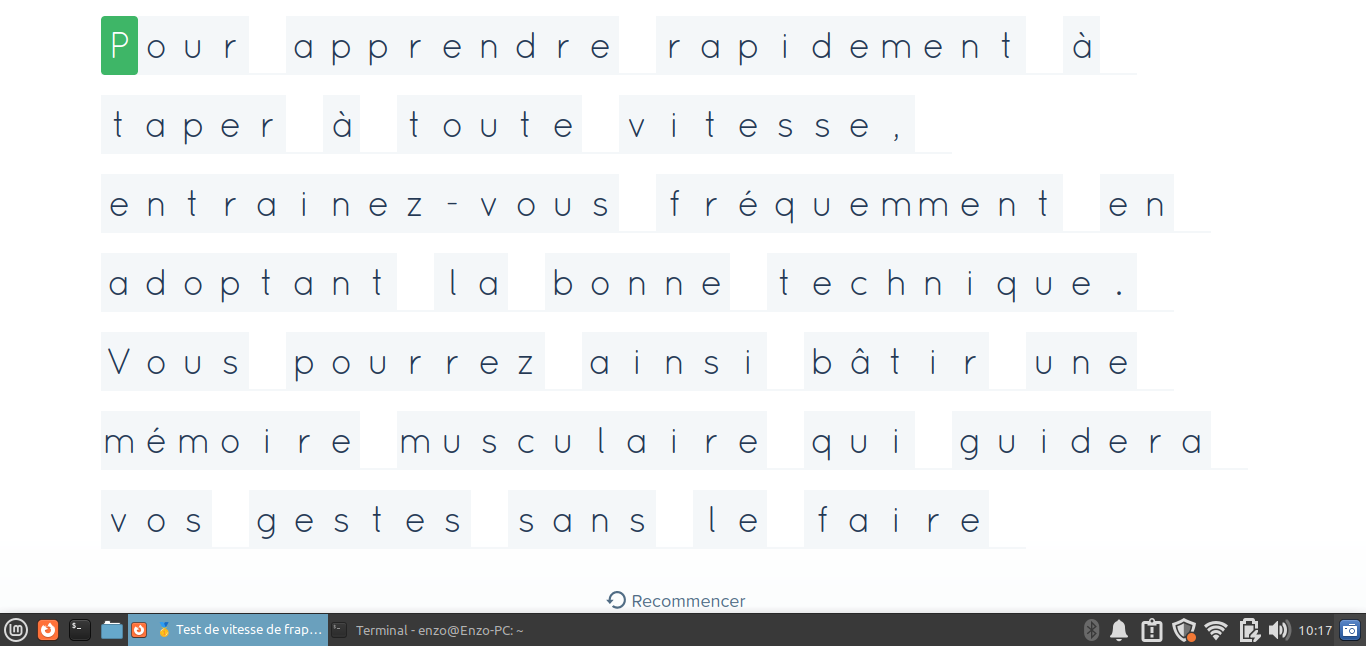
\includegraphics[width=\textwidth]{Image-TD-2/image_site_tap_touche2.png}
    \caption{Page pour effectuer le test de rapidité}
  \end{subfigure}
  \caption{Deux captures d'écran du site TapTouch}
\end{figure}

\vspace{0.3cm}

\begin{itemize}
  \item Essayer de masquer ses mains pour taper sans regarder
\end{itemize}

\vspace{0.3cm}

\begin{itemize}
  \item Inclure quelques résultats de rapidité.
\end{itemize}


\vspace{0.3cm}

Premier test effectué le 22/12/2022 : 

\begin{center}
  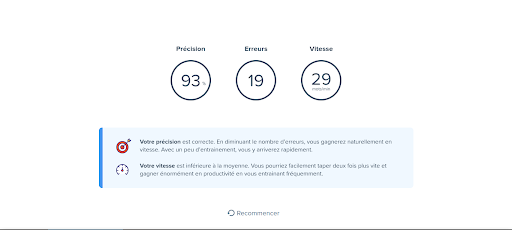
\includegraphics[width=10cm]{Image-TD-2/Premier_test.png}
\end{center}

\vspace{0.3cm}

\newpage

Deuxième test effectué le 23/12/2022 :

\begin{center}
  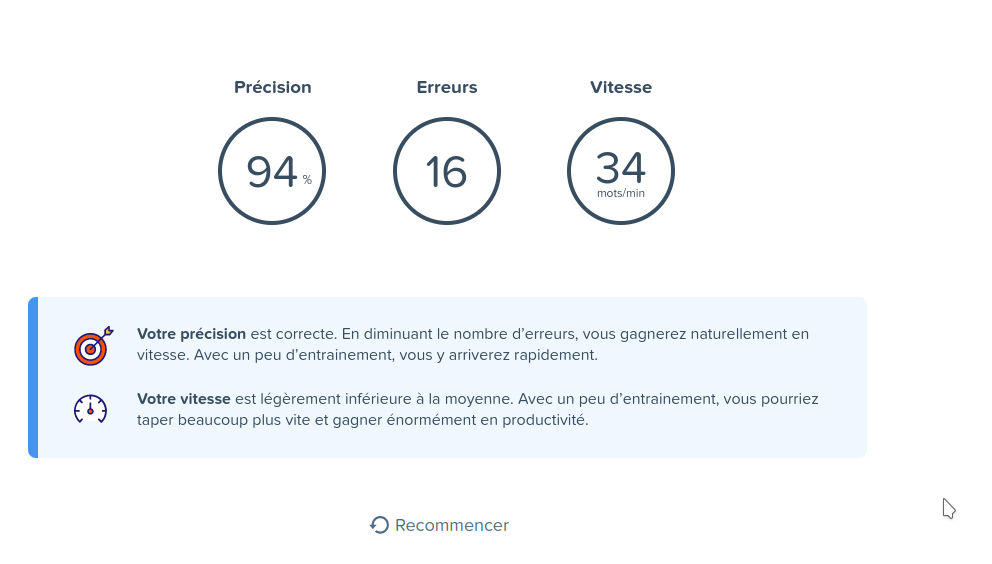
\includegraphics[width=10cm]{Image-TD-2/Deuxième_test.png}
\end{center}

\subsection{TD-3 : Vim et Emacs}

\begin{itemize}
  \item Effectuer les tutoriels pour Vim et Emacs :\\
  Vim : \texttt{vimtutor}\\
  Emacs : \texttt{emacs}, puis \texttt{Ctrl+H+T}
\end{itemize}

\vspace{0.3cm}

\begin{itemize}
  \item Paramétrer GNU Readline (le line editor par défault de bash) pour être en mode Emacs ou Vim
\end{itemize}

\vspace{0.3cm}

Une fois que j'ai effectué les deux tutoriels, je vais paramétrer GNU Readline en mode Vim. Pour cela, je vais utiliser la commande suivante :

\vspace{0.3cm}

\texttt{export EDITOR=vim}

\vspace{0.3cm}

Après, pour l'avoir de façon permanente, on peut ajouter cette ligne dans le fichier \texttt{~/.bashrc}.

\vspace{0.3cm}

\begin{itemize}
  \item Tester les deux 2 modes, en choisir un
\end{itemize}

\vspace{0.3cm}

J'ai testé ces deux modes et j'ai choisi d'utiliser Vim.

\vspace{0.3cm}

\begin{itemize}
  \item Paramétrer Emacs ou Vim comme étant éditeur par défault en plus du mode Readline.
\end{itemize}

\vspace{0.3cm}

Pour qu'il soit permanent, j'ai ajouté la ligne suivante dans le fichier bashrc, comme ci-dessous :

\vspace{0.3cm}

\begin{center}
  
\includegraphics[width=10cm]{Image-TD-3/Ajout-ligne-bashrc.png}
\end{center}

\newpage

  \subsection{TD-4 : Commande history}

\begin{itemize}
  \item Regarder votre history
\end{itemize}

\vspace{0.3cm}

Voici ci-dessous, une capture d'écran de mon history : 

\begin{center}
  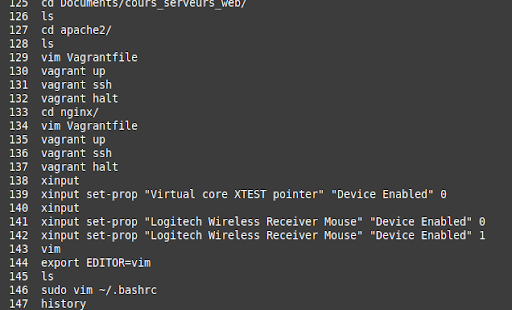
\includegraphics[width=10cm]{Image-TD-4/history.png}
\end{center}

\vspace{0.3cm}

\begin{itemize}
  \item Y a-t-il des informations sensible ? Comment y remédier ?
\end{itemize}

\vspace{0.3cm}

Oui, il peut y avoir des informations sensibles dans la commande history, telles que des mots de passe, etc. Pour remédier à cela, nous pouvons utiliser un autre interpréteur de commande, tel que ZSH.

\vspace{0.3cm}

\begin{itemize}
  \item Un employé de longue date semble avoir un \texttt{history} très court, quelle sont les causes possibles ?\\
  \vspace{0.3cm}
  ~ cat ~/.bash\_history\\
  \vspace{0.3cm}
  sudo apt install curl zsh git\\
  \vspace{0.3cm}
  sh -c "(curl -fsSL https://raw.github.com/ohmyzsh/ohmyzsh/master/tools/install.sh)" 
\end{itemize}

\vspace{0.3cm}

On peut constater que cet employé a utilisé un autre interpréteur de commande, qui est ZSH, en le combinant avec OHMYZSH. Par conséquent, on ne peut plus voir son historique dans bash_history.

\vspace{0.3cm}

\begin{itemize}
  \item Nos history sont souvent pollués par beaucoup de ls, cd, pwd ... Ces commandes sont tellement courtes que les taper entièrement est plus rapide. On veut éviter qu'elles n'apparaissent dans les résultats de recherche de l'history, comment faire ?
\end{itemize}

\vspace{0.3cm}

Pour éviter d'avoir certaines commandes dans notre historique, on peut ajouter l'option \texttt{HISTIGNORE} dans le fichier bashrc.

\vspace{0.3cm}

\begin{center}
  
\includegraphics[width=10cm]{Image-TD-4/HISTIGNORE.png}
\end{center}

\vspace{0.3cm}

\newpage

Voici le resulat ci-dessous : 

\vspace{0.3cm}

\begin{figure}[h]
  \centering
  \begin{subfigure}{0.45\textwidth}
    \centering
    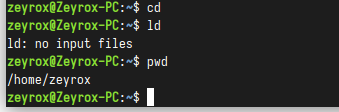
\includegraphics[width=\textwidth]{Image-TD-4/commande_test.png}
    \caption{Quelque commande pour tester HISTIGNORE}
  \end{subfigure}
  \vspace{0.9cm} % Espace verticale entre les images
  \begin{subfigure}{0.45\textwidth}
    \centering
    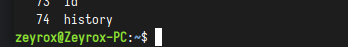
\includegraphics[width=\textwidth]{Image-TD-4/history1.png}
    \caption{Résultat dans history}
  \end{subfigure}
  \caption{Deux captures d'écran montrant un test de HISTIGNORE}
\end{figure}

\subsection{TD-5 : Alias}

\begin{itemize}
  \item Il est possible de créer des alias avec des arguments à l'aide des bash functions : 
\end{itemize}

\vspace{0.3cm}

\begin{itemize}
  \item Écrire une fonction bash "mkcd" qui crée le dossier "mondossier" puis navigue dedans.
\end{itemize}

\vspace{0.3cm}

Voici ci-dessous les étapes pour créer une bash function nommée mkcd :

\vspace{0.3cm}

\begin{center}
  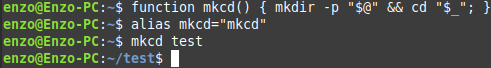
\includegraphics[width=10cm]{Image-TD-5/mkcd.png}
\end{center}

\vspace{0.3cm}

\begin{itemize}
  \item Ecrire une bash function gitemergency qui add, commit, et push tout son travail sur l'origine, permettant de ne rien perdre en cas d'alerte d'incendie.
\end{itemize}

\vspace{0.3cm}

Voici ci-dessous les étapes pour créer une bash function gitemergency :

\vspace{0.3cm}

\begin{center}
  
\includegraphics[width=14cm]{Image-TD-5/gitemergency.png}
\end{center}

\newpage

\subsection{TD-8 : Raccourci ZSH}

\vspace{0.3cm}

\begin{itemize}
  \item Dans zsh, créer un raccourci \texttt{Ctrl + Shift + A} :\\
  Lance les services apache et mariadb\\
  Log dans le terminal quand tout est lancé\\
  Ce reccourci est un interrupteur : apache et mariadb s'arrêtent si j'appuie à nouveau dessus.
\end{itemize}

\vspace{0.3cm}

Pour répondre à la question, nous allons tout d'abord créer un script bash comme ci-dessous :

\vspace{0.3cm}

\begin{center}
  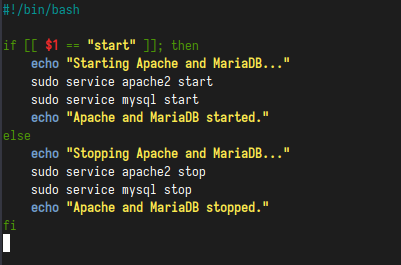
\includegraphics[width=7cm]{Image-TD-8/Sevices.png}
\end{center}

\vspace{0.3cm}

Maintenant que nous avons créé le script .sh, nous allons créer deux fonctions dans le fichier .zshrc pour faire fonctionner le script comme ci-dessous :

\vspace{0.3cm}

\begin{center}
  \includegraphics[width=7cm]{Image-TD-8/fonction\_zsh.png}
\end{center}

\vspace{0.3cm}

Maintenant que nous avons créé les deux fonctions, nous allons les combiner avec des touches dans le fichier .zshrc comme ci-dessous :

\vspace{0.3cm}

\begin{center}
  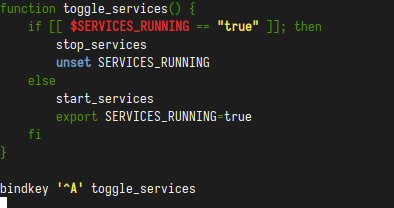
\includegraphics[width=7cm]{Image-TD-8/bindkey.png}
\end{center}

\vspace{0.3cm}

Il ne nous reste plus qu'à utiliser la commande \texttt{source ~/.zshrc} pour que les modifications soient prises en compte.

\newpage

  \subsection{TD-9 : Terminaux}

\vspace{0.3cm}

\begin{itemize}
  \item Installez et essayer 3+ émulateur de terminaux parmis la liste précédente : 
\end{itemize}

\vspace{0.3cm}

Pour ma part, je vais installer Terminator, Kitty et Tillix. Les installations des différents terminaux sous Debian sont ci-dessous :

\vspace{0.3cm}

Terminator : sudo apt-get install terminator

\vspace{0.3cm}

Image de Terminator : 

\vspace{0.3cm}

\begin{center}
  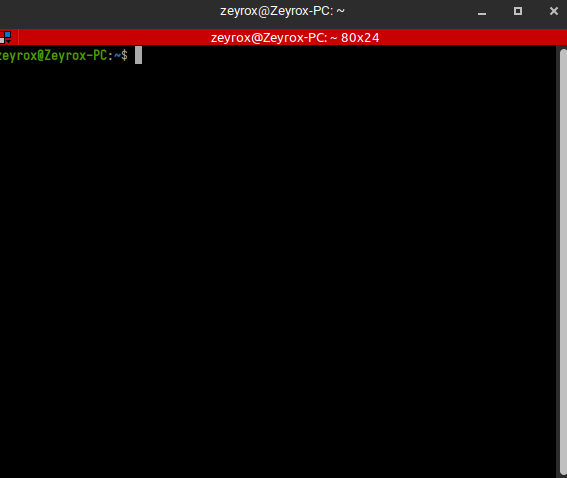
\includegraphics[width=7cm]{Image-TD-9/terminator.png}
\end{center}

\vspace{0.3cm}

Kitty: sudo apt-get install kitty

\vspace{0.3cm}

Image de Kitty : 

\vspace{0.3cm}

\begin{center}
  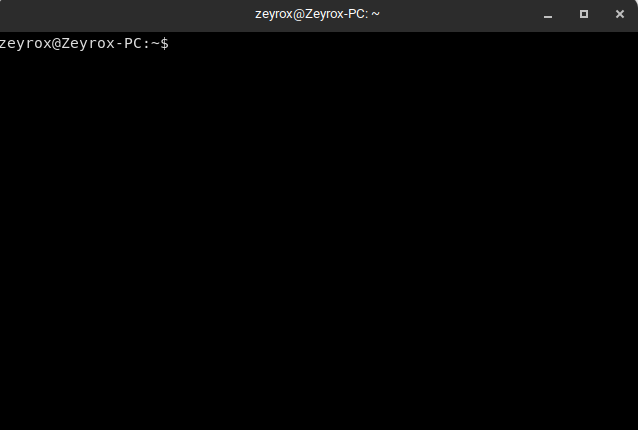
\includegraphics[width=7cm]{Image-TD-9/Kitty.png}
\end{center}

\newpage

\vspace{0.3cm}

Tilix: sudo apt-get install tilix

\vspace{0.3cm}

Image de Tilix : 

\vspace{0.3cm}

\begin{center}
  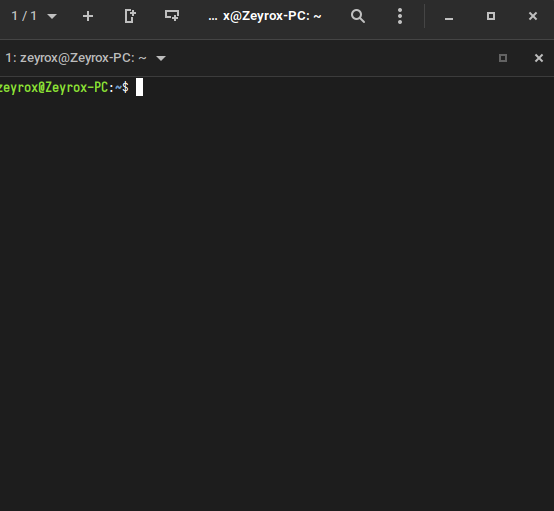
\includegraphics[width=7cm]{Image-TD-9/Tilix.png}
\end{center}

\vspace{0.3cm}

\begin{itemize}
  \item Choisir un terminal et justifier pourquoi \\
  Focntionnalitès\\
  Rapidité\\
  Documentation/Ecosystème
\end{itemize}

\vspace{0.3cm}

J'ai décidé de choisir Terminator car il offre beaucoup de possibilités. Au niveau des fonctionnalités, Terminator permet d'avoir plusieurs terminaux dans un seul terminal (multiplexage). On peut créer des onglets, définir des raccourcis et bien plus encore.

\vspace{0.3cm}

Ensuite, en ce qui concerne la rapidité, Terminator est un terminal très rapide et réactif.

\vspace{0.3cm}

Et pour finir, Terminator a une communauté très active et il est très bien documenté. Donc on peut conclure que dans l'ensemble, Terminator est un bon choix de terminal en raison de ses fonctionnalités, de sa rapidité et de sa très bonne documentation. C'est pour cela que j'ai décidé d'utiliser Terminator.

\vspace{0.3cm}

Et de mon point de vue, j'ai toujours utilisé Terminator car je trouve qu'il est facile à utiliser et une fois que l'on connaît les différentes combinaisons de touches, il peut devenir très puissant.

\vspace{0.3cm}

\begin{itemize}
  \item Désinstaller les autres terminaux
\end{itemize}

\vspace{0.3cm}

Pour désinstaller les autres terminaux, nous allons utiliser la commande suivante : 

\vspace{0.3cm}

sudo apt-get remove (le nom de terminal). Par exemple : sudo apt-get remove tilix.




\newpage

\section{Client SSH}

  \subsection{TD-1-SSH : Utilisation SSH}

\begin{itemize}
  \item Récupérer et démarrer l'environnement Vagrant sur arche ?
\end{itemize}

\vspace{0.3cm}

Pour ce nouveau TD, nous allons utiliser Vagrant pour utiliser SSH. Pour ce faire, nous allons télécharger depuis Arche le fichier Vagrant. Une fois que le fichier Vagrant est téléchargé, nous allons exécuter la machine Vagrant avec la commande ci-dessous :

\vspace{0.3cm}

\begin{center}
  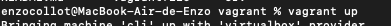
\includegraphics[width=7cm]{Image-TD-SSH-1/vagrant_up.png}
\end{center}

\vspace{0.3cm}

Une fois que la commande est terminer, on doit avoir ceci comment message qui indique que les machine sont bien démarrer : 

\vspace{0.3cm}

\begin{center}
  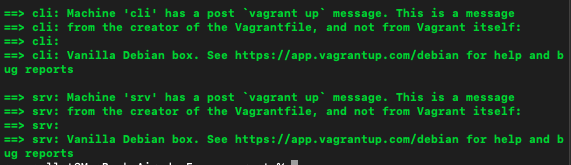
\includegraphics[width=7cm]{Image-TD-SSH-1/Machine.png}
\end{center}

\vspace{0.3cm}

\begin{itemize}
  \item Se connecter à la machine srv avec les utilisateurs alice, bob et carole sans utiliser vagrant ssh ?
\end{itemize}

\vspace{0.3cm}

Pour se connecter à la machine srv avec les utilisateurs alice, bob et carole sans utiliser vagrant ssh, nous allons utiliser la commande suivante : 

\vspace{0.3cm}

Connexion à l'utilisateur alice en ssh  : 

\vspace{0.3cm}

\begin{figure}[h]
  \centering
  \begin{subfigure}{0.30\textwidth}
    \centering
    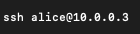
\includegraphics[width=\textwidth]{Image-TD-SSH-1/SSH-Alice.png}
    \caption{Connexion SSH avec l'utilisatrice Alice}
  \end{subfigure}
  \vspace{0.9cm} % Espace verticale entre les images
  \begin{subfigure}{0.45\textwidth}
    \centering
    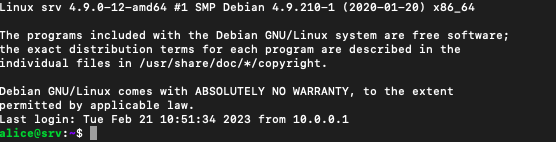
\includegraphics[width=\textwidth]{Image-TD-SSH-1/Connexion-SSH-Alice.png}
    \caption{Connexion Réussie avec l'utilisatrice Alice}
  \end{subfigure}
  \caption{Deux captures d'écran montrants une connexion en ssh au serveur srv avec l'utilisatrice Alice}
\end{figure}

\vspace{0.3cm}

Maintenant que nous avons réussi à nous connecter au serveur "srv" avec l'utilisateur "Alice", nous allons faire la même chose pour les deux autres utilisateurs.

\vspace{0.3cm}

\newpage

\vspace{0.3cm}

Connexion à l'utilisateur bob en ssh  : 

\vspace{0.3cm}

\begin{figure}[h]
  \centering
  \begin{subfigure}{0.30\textwidth}
    \centering
    
\includegraphics[width=\textwidth]{Image-TD-SSH-1/SSH-Bob.png}
    \caption{Connexion SSH avec l'utilisateur Bob}
  \end{subfigure}
  \vspace{0.9cm} % Espace verticale entre les images
  \begin{subfigure}{0.45\textwidth}
    \centering
    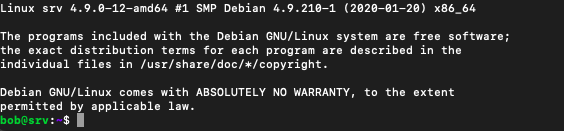
\includegraphics[width=\textwidth]{Image-TD-SSH-1/Connexion-SSH-Bob.png}
    \caption{Connexion Réussie avec l'utilisateur Bob}
  \end{subfigure}
  \caption{Deux captures d'écran montrants une connexion en ssh au serveur srv avec l'utilisateur Bob}
\end{figure}

\vspace{0.3cm}

Connexion à l'utilisateur carol en ssh  : 

\vspace{0.3cm}

\begin{figure}[h]
  \centering
  \begin{subfigure}{0.30\textwidth}
    \centering
    
\includegraphics[width=\textwidth]{Image-TD-SSH-1/SSH-Carol.png}
    \caption{Connexion SSH avec l'utilisatrice Carol}
  \end{subfigure}
  \vspace{0.9cm} % Espace verticale entre les images
  \begin{subfigure}{0.45\textwidth}
    \centering
    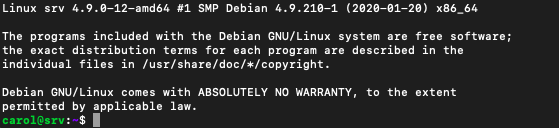
\includegraphics[width=\textwidth]{Image-TD-SSH-1/Connexion-SSH-Carol.png}
    \caption{Connexion Réussie avec l'utilisatrice Carol}
  \end{subfigure}
  \caption{Deux captures d'écran montrants une connexion en ssh au serveur srv avec l'utilisatrice Carol}
\end{figure}

\vspace{0.3cm}

\newpage

\vspace{0.3cm}

\begin{itemize}
  \item Vérifier qu'on est bien sur la machine Vagrant et pas en local ?
\end{itemize}

\vspace{0.3cm}

Pour verifier que nous somme bien sur la machine vagrant et non en local, nous allons utiliser la commande suivante : 

\vspace{0.3cm}

\begin{center}
  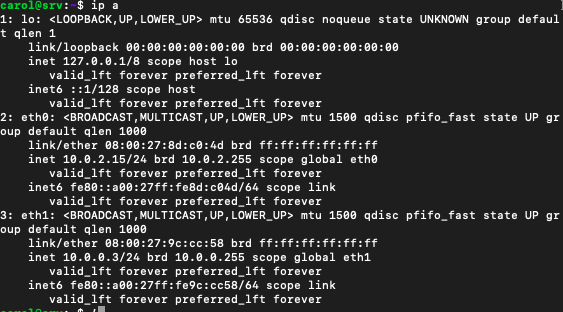
\includegraphics[width=7cm]{Image-TD-SSH-1/Commande-IPA.png}
\end{center}

\vspace{0.3cm}

On peut constater qu'au niveau des adresses IP, nous avons celle du serveur "srv", donc nous sommes bien sur la machine "vagrant".

\vspace{0.3cm}

\begin{itemize}
  \item Consulter l' history local, que remarque-t-on ?
\end{itemize}

\vspace{0.3cm}

Voici, ci-dessous l'history local : 

\vspace{0.3cm}

\begin{center}
  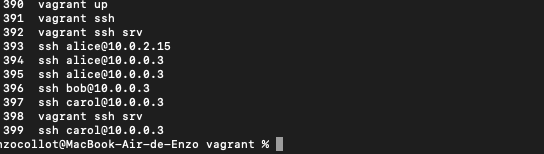
\includegraphics[width=7cm]{Image-TD-SSH-1/History-Local.png}
\end{center}

\vspace{0.3cm}

On peut constater que nous ne voyons pas les mots de passe que nous avons entrés pour nous connecter au serveur srv avec un utilisateur.


\subsection{TD-2-SSH : Authentification Publique}

\vspace{0.3cm}

\begin{itemize}
  \item Créer une paire de clés privée et publique à l'aide de ssh-keygen ?
\end{itemize}

Pour cette nouvelle étape, nous allons créer une paire de clés privée et publique à l'aide de ssh-keygen. Donc voici les étape ci-dessous pour le faire : 

\vspace{0.3cm}

Pour commencer, nous allons ouvrie un terminal est taper la commande suivante  : 

\vspace{0.3cm}

\begin{center}
  
\includegraphics[width=7cm]{Image-TD-SSH-2/ssh-keygen.png}
\end{center}

\vspace{0.3cm}

Ensuite, il nous demande à quel emplacement nous voulons enregistrer notre clé. Nous laissons par défaut :

\vspace{0.3cm}

\begin{center}
  
\includegraphics[width=7cm]{Image-TD-SSH-2/Emplacement-cle.png}
\end{center}

\vspace{0.3cm}

\newpage


Ensuite, il nous demande une passphrase. Vous pouvez en indiquer une, mais j'ai laissé par défaut. Une fois que c'est fini, vous devez avoir cela qui devrait apparaître :

\vspace{0.3cm}

\begin{center}
  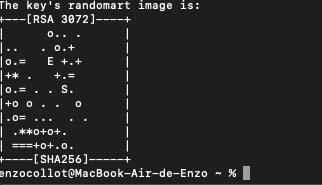
\includegraphics[width=7cm]{Image-TD-SSH-2/Génération-cle.png}
\end{center}

\vspace{0.3cm}

Voila, nous avons générer une clé rsa.

\vspace{0.3cm}

\begin{itemize}
  \item Utiliser la commande ssh-copy-id pour déposer la clé publique sur le compte alice@cli . Vérifier qu'on peut maintenant se connecter sans mot de passe ?
\end{itemize}

\vspace{0.3cm}

Pour cette nouvelle étape, nous allons utiliser la commande ssh-copy-id pour déposer la clé publique sur le compte alice@cli. Pour ce faire, nous allons utiliser la commande suivantes : 

\vspace{0.3cm}

\begin{center}
  
\includegraphics[width=7cm]{Image-TD-SSH-2/ssh-copy-id.png}
\end{center}

\vspace{0.3cm}

Une fois que nous avons entrée la commande, il va nous demander le mot de passe de Alice. Une fois le mots de passe entrer, nous avons ceci qui apparaît : 

\vspace{0.3cm}

\begin{center}
  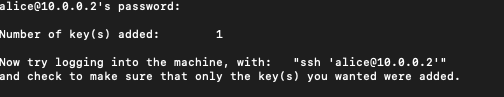
\includegraphics[width=7cm]{Image-TD-SSH-2/key-add.png}
\end{center}

\vspace{0.3cm}

Maintenant, on peut ce connecter en compte d'alice sur le serveur cli sans rentrer son mots de passe.

\vspace{0.3cm}

\begin{itemize}
  \item Déposer manuellement la clé publique sur le compte bob@cli \\
  Les nouvelles clés créés sont dans ~/.ssh\\
  Les clées autorisées à se connecter au serveur sont dans ~/.ssh/authorized\_keys
\end{itemize}

\vspace{0.3cm}

Pour déposer manuellement la clé publique sur le compte bob@cli, vous pouvez suivre les étapes ci-dessous : 

\vspace{0.3cm}

Pour commencer, nous allons afficher le contenue de notre clé publique et le copier avec la commande suivante : 

\vspace{0.3cm}

\begin{center}
  \includegraphics[width=7cm]{Image-TD-SSH-2/Clé-pub.png}
\end{center}

\vspace{0.3cm}

\newpage

Une fois que nous avons copier la clé publique, nous allons nous connecter au compte de bob@cli avec la commande suivante : \\

\texttt{ssh bob@cli}

\vspace{0.3cm}

Une fois connecter sur le compte, nous allons verifier si le dossier .ssh existe. Si il existe pas, nous le créons avec la commande suivante : \\

\texttt{mkdir ~/.ssh}

\vspace{0.3cm}

Ensuite, on tape la commande suivante pour créer ou ouvrir le fichier "authorized\_keys" : \\

\texttt{nano ~/.ssh/authorized\_keys}

\vspace{0.3cm}

Maintenant, on copie le contenue de la clé publique dans le fichier comme ci-dessous  : 

\vspace{0.3cm}

\begin{center}
  \includegraphics[width=7cm]{Image-TD-SSH-2/clé-pub-bob.png}
\end{center}

\vspace{0.3cm}

Une fois que nous avons enregistrer le fichier, c'est bon, on peut ce connecter au compte de bob@cli sans taper le mot de passe avec la commande suivante : \\  

\texttt{ssh -i ~/.ssh/id\_rsa.pub bob@cli}


\subsection{TD-3-SSH : Connexion Automatique}

\begin{itemize}
  \item Purger le fichier ~/.ssh/known\_hosts si nécessaire ?
\end{itemize}

\vspace{0.3cm}

Pour cette nouvelle étape, nous allons purger le fichier ~/.ssh/known\_hosts avec la commande suivante : 

\texttt{sudo rm known\_host}

\vspace{0.3cm}

\begin{itemize}
  \item A l'aide de ssh-keygen et ssh-keyscan , ajouter la clé publique du serveur srv manuellement, décrire les étapes. \\
  Votre client SSH ne doit pas demander d'ajouter la clé publique du serveur à la première connexion.
\end{itemize}

\vspace{0.3cm}

Voici les étapes pour ajouter manuellement la clé publique du serveur srv au fichier known\_hosts à l'aide des commandes ssh-keygen et ssh-keyscan :

\vspace{0.3cm}

Tout d'abord, on va utiliser la commande ssh-keyscan pour récupérer la clé publique du serveur srv. Dans un terminal, on va utiliser la commande suivante : 

\texttt{ssh-keyscan 10.0.0.3 >> ~/.ssh/known\_hosts}

\vspace{0.3cm}

\begin{center}
  
\includegraphics[width=7cm]{Image-TD-SSH-3/ssh-keyscan.png}
\end{center}

\vspace{0.3cm}

\begin{center}
  \includegraphics[width=7cm]{Image-TD-SSH-3/résultat-ssh-keyscan.png}
\end{center}

\vspace{0.3cm}

\newpage

Ensuite, on va utiliser la commande ssh-keygen pour générer une paire de clés SSH (une clé publique et une clé privée) sur l'ordinateur local. Dans le même terminal, tapez la commande suivante :

\texttt{ssh-keygen}

\vspace{0.3cm}

\begin{center}
  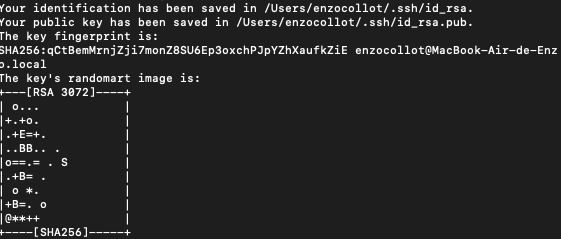
\includegraphics[width=7cm]{Image-TD-SSH-3/Génération-key.png}
\end{center}


\vspace{0.3cm}

Une fois que nous avons généré une paire de clés SSH, nous allons  copier la clé publique sur le serveur srv. Pour ce faire, nous allons entrer la commande suivante dans le terminal :

\texttt{ssh-copy-id -i ~/.ssh/id/\_rsa.pub user@srv} 

\vspace{0.3cm}

Ici, user@srv on remplace par les utilisateur sur le serveur srv. un petit exemple ci-dessous  : 

\vspace{0.3cm}

\begin{center}
  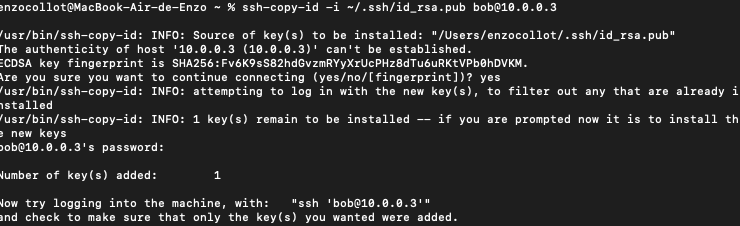
\includegraphics[width=7cm]{Image-TD-SSH-3/ssh-copy-id.png}
\end{center}

\vspace{0.3cm}

Voila, maintenant, on peut se connecter automatique avec l'utilisateur bob au serveur srv.

\vspace{0.3cm}

\begin{itemize}
  \item Créer un fichier de configuration pour SSH, vous permettant de vous connecter sur le compte bob@cli en tapant ssh bc.
\end{itemize}

\vspace{0.3cm}

Voici les étapes pour créer un fichier de configuration pour SSH qui permettra de se connecter au compte bob@cli en tapant simplement ssh bc :

\vspace{0.3cm}

Pour commencer, nous allons tapez la commande suivante pour créer un nouveau fichier de configuration SSH :

\texttt{nano ~/.ssh/config}

\vspace{0.3cm}

\begin{center}
  
\includegraphics[width=7cm]{Image-TD-SSH-3/fichier-config.png}
\end{center}

\vspace{0.3cm}

Dans le fichier de configuration, ajoutez les lignes suivantes :

\vspace{0.3cm}

\begin{center}
  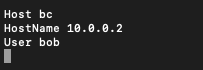
\includegraphics[width=7cm]{Image-TD-SSH-3/ligne-conf.png}
\end{center}

\vspace{0.3cm}

\newpage

Une fois que nous avons mis les informations dans le fichier de configuration, nous pouvons nous connecter comme ci-dessous : 

\vspace{0.3cm}

\begin{figure}[h]
  \centering
  \begin{subfigure}{0.30\textwidth}
    \centering
    \includegraphics[width=\textwidth]{Image-TD-SSH-3/Connexion-SSH-Complétion.png}
    \caption{Connexion SSH en utilisant l'auto-complétion}
  \end{subfigure}
  \vspace{0.9cm} % Espace verticale entre les images
  \begin{subfigure}{0.45\textwidth}
    \centering
    \includegraphics[width=\textwidth]{Image-TD-SSH-3/Connexion-réussite.png}
    \caption{Connexion réussite avec l'utilisateur Bob}
  \end{subfigure}
  \caption{Deux captures d'écran montrants une connexion en ssh au serveur srv avec l'utilisateur bob en utilisant l'auto-complétion}
\end{figure}

\vspace{0.3cm}

\subsection{TD-4-SSH : SFTP-SSHFS}

\begin{itemize}
  \item Vérifiez que vous arrivez à vous connecter au compte alice@cli en utilisant SFTP. \\ 
  Copiez-y un fichier par SFTP, puis récupérez un autre fichier. ?
\end{itemize}

\vspace{0.3cm}

Pour cette nouvelle étape, nous allons nous connecter avec l'utilisateur alice en utilisant SFTP. Pour ce faire, nous allons ouvrir un terminal et taper la commande suivante : 

\texttt{sftp alice@10.0.0.2}

\vspace{0.3cm}

\begin{center}
  
\includegraphics[width=7cm]{Image-TD-SSH-4/commande-sftp.png}
\end{center}

\vspace{0.3cm}

\begin{center}
  
\includegraphics[width=7cm]{Image-TD-SSH-4/connexion-sftp.png}
\end{center}

\vspace{0.3cm}

On peut constater que nous somme bien connecter en sftp au serveur cli avec l'utilisateur Alice.

\vspace{0.3cm}

Maintenant que nous somme connecté, nous allons copier un fichier de notre machine local vers la machine virutel. Pour ce faire, nous allons crée un fichier texte et l'envoyer sur le serveur. Voici les étapes ci-dessous : 

\vspace{0.3cm}

Pour commencer, nous allons crée un fichier texte avec la commande suivante  : 

\vspace{0.3cm}

\begin{center}
  \includegraphics[width=7cm]{Image-TD-SSH-4/création-fichier.png}
\end{center}

\vspace{0.3cm}

\newpage

\vspace{0.3cm}

Une fois que nous avons crée le fichier, on se reconnecte au serveur avec la commande que nous avons vue précédement. Une fois connecter, nous allons utiliser la commande suivante : 

\vspace{0.3cm}

\begin{center}
  
\includegraphics[width=7cm]{Image-TD-SSH-4/fichier-envoyer.png}
\end{center}

\vspace{0.3cm}

\begin{center}
  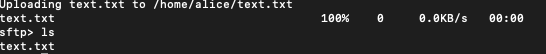
\includegraphics[width=7cm]{Image-TD-SSH-4/commande-reussite.png}
\end{center}

\vspace{0.3cm}

On peut constater que notre fichier à bien était envoyé sur le serveur. 

\vspace{0.3cm}

Maintenant que nous avons envoyer un fichier de notre machine local vers la machine virtuelle, nous allons prendre un fichier de la machine virtuelle et nous allons le télécherger sur la machine local. Pour ce faire, nous allons utiliser la commande suivante : 

\vspace{0.3cm}

\begin{center}
  
\includegraphics[width=7cm]{Image-TD-SSH-4/commande-puts.png}
\end{center}

\vspace{0.3cm}

\begin{center}
  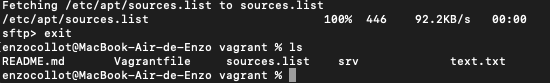
\includegraphics[width=7cm]{Image-TD-SSH-4/commande-puts-2.png}
\end{center}

\vspace{0.3cm}

On peut constater que nous avons bien reçus le fichier du serveur sur notre machine local.

\vspace{0.3cm}

\begin{itemize}
  \item Vérifiez que vous arrivez à vous connecter au compte alice@cli avec SSHFS. \\
  Éditez un fichier distant avec un éditeur graphique (par exemple GVIM)
\end{itemize}

\vspace{0.3cm}

\begin{itemize}
    \item Vérifiez que la modification est bien répercutée sur la machine virtuelle alice@cli.
\end{itemize}

\vspace{0.3cm}

Pour cette nouvelle étape, je vais répondre au deux question en même temps. Pour commencer, nous allons nous connecter au compte alice@cli avec SSHFS. Pour ce faire, nous allons utiliser la commande suivante : 

\vspace{0.3cm}

\begin{center}
  \includegraphics[width=7cm]{Image-TD-SSH-4/sshfs.png}
\end{center}

\vspace{0.3cm}

Verfication du montage dans le dossier /tmp/alicecli : 

\vspace{0.3cm}

\begin{center}
  \includegraphics[width=7cm]{Image-TD-SSH-4/montage-sshfs.png}
\end{center}

\vspace{0.3cm}

On peut constater que le montage à bien était réalisé. 

\newpage

\vspace{0.3cm}

Maintenant, nous allons modifier un fichier avec vim et regarder si les modification se repercute quand on se connecte directement au serveur. Pour ce faire, nous allons créé un fichier avec vim et mettre des informations dedans comme ci-dessous  : 

\vspace{0.3cm}

\begin{center}
  \includegraphics[width=7cm]{Image-TD-SSH-4/Modification-fichier-vim.png}
\end{center}

\vspace{0.3cm}

Une fois que nous avons créé et modifié le fichier, nous allons nous connecter au serveur avec alice comme ci-dessous : 

\vspace{0.3cm}

\begin{center}
  \includegraphics[width=7cm]{Image-TD-SSH-4/connexion-ssh.png}
\end{center}

\vspace{0.3cm}

Une fois que nous somme connecter, nous allons regarder les information dans le fichier comme ci-dessous  : 


\vspace{0.3cm}

\begin{center}
  \includegraphics[width=7cm]{Image-TD-SSH-4/verfication-fichier.png}
\end{center}

\vspace{0.3cm}

On peut constater que notre fichier à bien était modifier.

\newpage

\subsection{TD-5-SSH : Tunnel SSH}

\vspace{0.3cm}

\begin{itemize}
  \item Créer un tunnel SSH entre votre poste et srv à travers la machine cli ?
\end{itemize}

\vspace{0.3cm}

Pour cette nouvelle étape, nous allons crée un tunnel SSH entre mon poste et srv à travers la machine cli. Pour ce faire, nous allons ouvrir un termnial et taper la commande ci-dessous : 

\vspace{0.3cm}

\begin{center}
  \includegraphics[width=7cm]{Image-TD-SSH-5/port-local.png}
\end{center}

\vspace{0.3cm}

Maintenant que nous avons crée notre tunnel ss, nous pouvons passer à la suite.

\vspace{0.3cm}

\begin{itemize}
  \item Tester en ouvrant un navigateur sur votre poste local à l'adresse http://localhost:8000/cgi-bin/test1.cgi.
\end{itemize}

\vspace{0.3cm}

\begin{itemize}
  \item Pour srv , le navigateur devrait donc provenir de cli , et pas de votre poste local. \\
  Si c'est OK, vous devriez avoir le message « OK : la connexion est bien établie depuis l’adresse de la VM cli »
\end{itemize}

\vspace{0.3cm}

Ici, je vais repondre directement au deux question, maintenant nous allons tester la connexion en nous rendant à l'adresse suivante : http://localhost:8000/cgi-bin/test1.cgi. \\

Voici ci-dessous, le résultat de la page : 

\vspace{0.3cm}

\begin{center}
  \includegraphics[width=7cm]{Image-TD-SSH-5/Connexion-Cli.png}
\end{center}

\vspace{0.3cm}

On peut constater que nous avons bien le message « OK : la connexion est bien établie depuis l’adresse de la VM cli ». Donc notre tunnel SSH fonctionne correctement.

\newpage

\subsection{TD-6-SSH : Tunnel-Tsock}

\vspace{0.3cm}

\begin{itemize}
  \item Se connecter en SSH sur srv .
\end{itemize}

\vspace{0.3cm}

Pour cette nouvelle étape, nous allons nous connecter au serveur srv via SSH comme ci-dessous  : 

\vspace{0.3cm}

\begin{center}
  \includegraphics[width=7cm]{Image-TD-SSH-6/connexion-ssh-srv.png}
\end{center}

\vspace{0.3cm}

Maintenant que nous somme connecter au serveur srv, nous pouvons passer à la suite.

\vspace{0.3cm}

\begin{itemize}
  \item Se connecter à cli en permettant à cli d’accéder à srv via un tunnel accessible par le port 9000.
\end{itemize}

\vspace{0.3cm}

Pour ce connecter au serveur cli en permettant à cli d’accéder à srv via un tunnel accessible par le port 9000, nous allons crée un tunnel SSH comme ci-dessous : 

\vspace{0.3cm}

\begin{center}
  \includegraphics[width=7cm]{Image-TD-SSH-6/tunnel-ssh.png}
\end{center}

\vspace{0.3cm}

Maintenant que nous avons crée le tunnel SSH, nous allons passer à la suite. 

\vspace{0.3cm}

\begin{itemize}
  \item Vérifier que vous arrivez à accéder au serveur web : wget -nv -O - http://localhost:9000/cgi-bin/test2.cgi.
\end{itemize}

\vspace{0.3cm}

Pour verifier, nous allons utiliser la commande wget -nv -O - http://localhost:9000/cgi-bin/test2.cgi comme ci-dessous : 

\vspace{0.3cm}

\begin{center}
  \includegraphics[width=7cm]{Image-TD-SSH-6/commande-wget.png}
\end{center}

\vspace{0.3cm}

On peut constater que nous arrivons à accéder à la page web.

\vspace{0.3cm}

\newpage

\subsection{TD-7-SSH : X11 Forward}

\vspace{0.3cm}

\begin{itemize}
  \item Installer une application graphique sur cli (par exemple xclock ou xeyes ,disponibles dans le paquet x11-apps ), ainsi que xauth (disponible dans le paquet xauth ).
\end{itemize}

\vspace{0.3cm}

Pour cette nouvelle étape, nous allons une application graphique sur le serveur cli. Pour ce faire, nous allons nous connecter sur le serveur cli et installer les application suivante : 

\texttt{sudo apt-get install x11-apps} \\
\texttt{sudo apt-get install xauth}

\vspace{0.3cm}

Maintenant que nous avons installer ces deux paquets, nous pouvons passé à la suite.

\vspace{0.3cm}

\begin{itemize}
  \item Se connecter sur cli en activant le forwarding X11.
\end{itemize}

\vspace{0.3cm}

Pour ce connecter sur cli en activant le forwarding X11, nous allons utiliser la commande ci-dessous : 

\vspace{0.3cm}

\begin{center}
  \includegraphics[width=7cm]{Image-TD-SSH-7/SSH-Forwarding-X11.png}
\end{center}

\vspace{0.3cm}

Une fois que nous somme connecter, nous pouvons passer à la suite. 

\vspace{0.3cm}

\begin{itemize}
  \item Vérifier que vous pouvez lancer les applications graphiques installées et que les GUI s'affichent sur le poste local.
\end{itemize}

\vspace{0.3cm}

Nous allons lancer une application graphique via le terminal. Donc voici les étapes pour lancer l'application graphique : 

\vspace{0.3cm}

\begin{center}
  \includegraphics[width=7cm]{Image-TD-SSH-7/Commande-xeyes.png}
\end{center}

\vspace{0.3cm}

\begin{center}
  \includegraphics[width=7cm]{Image-TD-SSH-7/Application-X11.png}
\end{center}

\vspace{0.3cm}

Voila, nous avons reussi à lancer une application graphique X11 depuis le terminal.

\newpage

\subsection{TD-8-SSH : Rebonds SSH}

\vspace{0.3cm}

\begin{itemize}
  \item Configurer .ssh/config avec ProxyJump de manière à pouvoir rebondir automatiquement sur cli lorsque vous vous connectez à srv.
\end{itemize}

\vspace{0.3cm}

Dans cette nouvelle étape, nous allons configurer ProxyJump de manière à pouvoir rebondir automatiquement sur cli lorsque l'on se connecte à srv. Pour ce faire, nous allons crée et modifier le fichier config comme ci-dessous : 

\vspace{0.3cm}

\begin{center}
  \includegraphics[width=7cm]{Image-TD-SSH-8/nano-config.png}
\end{center}

\vspace{0.3cm}

\begin{center}
  \includegraphics[width=7cm]{Image-TD-SSH-8/ProxyJump.png}
\end{center}

\vspace{0.3cm}

Maintenant que nous avons configuer le fichier config, nous pouvons passer à la suite.

\vspace{0.3cm}

\begin{itemize}
  \item Vous pouvez utiliser la commande who pour vérifier de quelle adresse vous connectez.
\end{itemize}

\vspace{0.3cm}

Maintenant que nous avons configuer ProxyJump, nous allons nous connecter au serveur srv. Une fois connecter, nous allons utiliser la commande who ci-dessous : 

\vspace{0.3cm}

\begin{center}
  \includegraphics[width=7cm]{Image-TD-SSH-8/commande-who.png}
\end{center}

\vspace{0.3cm}

On peut constater que nous somme connecter au serveur srv en passant par le serveur cli. Donc le rebonds c'est bien effectué.

\vspace{0.3cm}

\begin{itemize}
  \item Idem en utilisant ProxyCommand au lieu de ProxyJump.
\end{itemize}

\vspace{0.3cm}

Pour cette nouvelle étape, nous allons utiliser ProxyCommand. Pour ce faire nous allons reprendre notre fichier config et le modifier comme ceci : 

\vspace{0.3cm}

\begin{center}
  \includegraphics[width=7cm]{Image-TD-SSH-8/ProxyCommand.png}
\end{center}

\vspace{0.3cm}

Maintenant que nous avons configuer le fichier config, nous pouvons passer à la suite.

\vspace{0.3cm}

\begin{itemize}
  \item Vous pouvez utiliser la commande who pour vérifier de quelle adresse vous connectez.
\end{itemize}

\vspace{0.3cm}

Maintenant que nous avons configuer ProxyCommand, nous allons nous connecter au serveur srv. Une fois connecter, nous allons utiliser la commande who ci-dessous : 

\vspace{0.3cm}

\begin{center}
  \includegraphics[width=7cm]{Image-TD-SSH-8/commande-who-2.png}
\end{center}

\vspace{0.3cm}

On peut constater que nous somme connecté au serveur srv en passant par le serveur cli. Donc le rebonds c'est bien effectué.

\newpage

\subsection{TD-9-SSH : Bonus SSH}

\vspace{0.3cm}

\begin{itemize}
  \item Vérifiez que vous pouvez couper une connexion SSH en utilisant une séquence d’échappement.
\end{itemize}

\vspace{0.3cm}

Pour cette nouvelle étape, nous allons verifier que l'on peut couper une connexion SSH en utilisant une séquence d’échappement. Pour ce faire, nous allons dans une fenêtre SSH et nous allons utiliser ce caractére d'échapement : 

\vspace{0.3cm}

\begin{center}
  \includegraphics[width=7cm]{Image-TD-SSH-9/echappement.png}
\end{center}

\vspace{0.3cm}

\begin{center}
  \includegraphics[width=7cm]{Image-TD-SSH-9/fin-de-conection.png}
\end{center}

\vspace{0.3cm}

On peut constater que nous avons reussie à mettre fin à la connexion SSH.

\vspace{0.3cm}

\begin{itemize}
  \item Installez screen sur cli. \\
  Connectez-vous-y \\
  Lancez un screen , puis une commande dans un screen . - Déconnectez-vous
  du screen et de cli . Vérifiez que vous pouvez vous reconnecter à cli et au
  screen , et retrouver votre commande en cours d’exécution.
\end{itemize}

\vspace{0.3cm}

Pour cette nouvelle étape, nous allons installer screen sur cli. Pour ce faire, nous connecter à cli et taper la commande ci-dessous : 

\texttt{sudo apt-get install screen}

\vspace{0.3cm}

Maintenant que nous avons installer screen, nous allons le lancer et taper une commande comme ci-dessous  : 

\vspace{0.3cm}

\begin{center}
  \includegraphics[width=7cm]{Image-TD-SSH-9/screen.png}
\end{center}

\vspace{0.3cm}

\begin{center}
  \includegraphics[width=7cm]{Image-TD-SSH-9/ping.png}
\end{center}

\vspace{0.3cm}

Maintenant que nous avons une commande en cours d'éxécution, nous allons quitter la session avec la combinaison de touche ci-dessous : 

\texttt{Ctrl + ad}

\newpage

\vspace{0.3cm}

Une fois que nous avons quitter le terminal screen, nous allons y retourner avec la commande ci-dessous : 

\vspace{0.3cm}

\begin{center}
  \includegraphics[width=7cm]{Image-TD-SSH-9/screen_r.png}
\end{center}

\vspace{0.3cm}

\begin{center}
  \includegraphics[width=7cm]{Image-TD-SSH-9/screen-return.png}
\end{center}

\vspace{0.3cm}

On peut constater que nous avons retrouver notre terminal comme nous l'avons quitter.

\vspace{0.3cm}

\begin{itemize}
  \item Idem avec tmux
\end{itemize}

\vspace{0.3cm}

Pour cette nouvelle étape, nous allons installer tmux sur cli. Pour ce faire, nous connecter à cli et taper la commande ci-dessous : 

\texttt{sudo apt-get install tmux}

\vspace{0.3cm}

Maintenant que nous avons installer tmux, nous allons le lancer et taper une commande comme ci-dessous  : 

\vspace{0.3cm}

\begin{center}
  \includegraphics[width=7cm]{Image-TD-SSH-9/tmux.png}
\end{center}

\vspace{0.3cm}

\begin{center}
  \includegraphics[width=7cm]{Image-TD-SSH-9/ping-tmux.png}
\end{center}

\vspace{0.3cm}

Maintenant que nous avons une commande en cours d'éxécution, nous allons quitter la session avec la combinaison de touche ci-dessous : 

\texttt{Ctrl + bd}

\newpage

\vspace{0.3cm}

Une fois que nous avons quitter le terminal screen, nous allons y retourner avec la commande ci-dessous : 

\vspace{0.3cm}

\begin{center}
  \includegraphics[width=7cm]{Image-TD-SSH-9/tmux-attach.png}
\end{center}

\vspace{0.3cm}

\begin{center}
  \includegraphics[width=7cm]{Image-TD-SSH-9/return-tmux.png}
\end{center}

\vspace{0.3cm}

On peut constater que nous avons retrouver notre terminal comme nous l'avons quitter.




\newpage

\section{Git}

\subsection{TD-1-Git : Initialisation Git}

\vspace{0.3cm}

\begin{itemize}
  \item Créer un nouveau répertoire et y initialiser un repository.
\end{itemize}

Pour cette nouvelle étape, nous allons créé un nouveaux répertoire et initialiser un repository. Pour ce faire, voici les étapes ci-dessous : 

\vspace{0.3cm}

\begin{figure}[h]
  \centering
  \begin{subfigure}{0.30\textwidth}
    \centering
    \includegraphics[width=\textwidth]{Image-TD-Git-1/new-directory.png}
    \caption{Création d'un repertoire pour git}
  \end{subfigure}
  \vspace{0.9cm} % Espace verticale entre les images
  \begin{subfigure}{0.45\textwidth}
    \centering
    \includegraphics[width=\textwidth]{Image-TD-Git-1/git-init.png}
    \caption{Initialisation d'un repository}
  \end{subfigure}
  \caption{Deux capture d'ecran montrant comment initialiser un repository}
\end{figure}

\vspace{0.3cm}

\begin{itemize}
  \item Y copier la configuration Vagrant des TD ssh (Vagrantfile + dossier srv).
\end{itemize}

Maintenant que nous avons initialiser notre repository, nous allons copier les fichiers demander dans la questions. Voici la commande pour copier les fichiers : 

\texttt{cp -r /chemin/Vagrantfile /chemin/td-git} \\
\texttt{cp -r /chemin/srv /chemin/td-git}

\vspace{0.3cm}

Un fois que l'on à copier les bons documents au bonne endroits, nous pouvons passez à la question suivante. 

\vspace{0.3cm}

\begin{itemize}
  \item Regarder les modifications détectées par git.
\end{itemize}

\vspace{0.3cm}

Pour regarder les informations détectées par git, nous allons utiliser la commande suivante : 

\texttt{git status}

\vspace{0.3cm}

\begin{center}
  \includegraphics[width=7cm]{Image-TD-Git-1/git-status.png}
\end{center}

\vspace{0.3cm}

\begin{itemize}
  \item Démarrer puis arrêter la configuration Vagrant.
\end{itemize}

Pour démarrer puis arrêter la configuration Vagrant, nous allons utiliser ses deux commande ci-dessous : \newline

Pour démarrer : 

\texttt{vagrant up}

Pour démarrer : 

\texttt{vagrant halt}

\vspace{0.3cm}

\newpage

\begin{itemize}
  \item Regarder à nouveau les modifications détectées par git.
\end{itemize}

Pour cette nouvelle étapes, nous allons regarder de nouveaux les modification détectées par git. Voici ci-dessous, les modification détectées par git : 

\vspace{0.3cm}

\begin{center}
  \includegraphics[width=7cm]{Image-TD-Git-1/git-status-2.png}
\end{center}

\vspace{0.3cm}

\begin{itemize}
  \item Que remarque-t-on ? Comment peut-on régler le problème ?
\end{itemize}

On peut constater que nous avons actuellement sur la branche master, des fichiers non suivie et qu'il n'y a pas eu de commit fait. \newline

Pour régler le probléme, il suffit à d'ajouter les fichier et de faire un commit tout en ignorant le dossier .vagrant.

\vspace{0.3cm}

\begin{itemize}
  \item Ajouter les fichiers Vagrant et commit les modifications.
\end{itemize}

Avant d'ajouter les fichiers Vagrant et commit les modifications, nous allons faire en sorte que git igonore le dossier .vagrant. \newline

Pour ce faire, nous allons créé un fichier .gitignore et ajouter la ligne .vagrant comme ci-dessous : 

\vspace{0.3cm}

\begin{center}
  \includegraphics[width=7cm]{Image-TD-Git-1/gitignore.png}
\end{center}

\vspace{0.3cm}

Maintenant que nous avons ignorer le dossier .vagrant, nous allons ajouter les fichiers Vagrant et commit les modifications. Voici les étapes ci-dessous : 

\vspace{0.3cm}

\begin{center}
  \includegraphics[width=7cm]{Image-TD-Git-1/git add.png}
\end{center}

Une fois que nous avons ajouter les fichiers Vagrant, nous allons crée un commit comme ci-dessous : 

\vspace{0.3cm}

\begin{center}
  \includegraphics[width=7cm]{Image-TD-Git-1/git commit.png}
\end{center}

\vspace{0.3cm}

Voila nous avons commit et ajouter les fichiers Vagrant.

\vspace{0.3cm}

\begin{itemize}
  \item Vérifier que le commit est bien présent et correct.
\end{itemize}

\vspace{0.3cm}

Pour verifier que le commit est bien présent et correct, nous allons utiliser la commande suivants : 

\texttt{git log}

\vspace{0.3cm}

\begin{center}
  \includegraphics[width=7cm]{Image-TD-Git-1/git-log.png}
\end{center}

\vspace{0.3cm}

On peut constater que notre commit est bien présent et correct.

\newpage

\subsection{TD-2-Git : Les branches}

\vspace{0.3cm}

\begin{itemize}
  \item Créer une nouvelle branche.
\end{itemize}

\vspace{0.3cm}

Dans cette nouvelle partie, nous allons créé une nouvelle branche. Pour ce faire, nous allons utiliser la commande suivante : 

\texttt{git checkout -b "nom-de-la-branche"}

\vspace{0.3cm}

\begin{center}
  \includegraphics[width=7cm]{Image-TD-Git-2/git-checkout.png}
\end{center}

\vspace{0.3cm}

\begin{itemize}
  \item Dans le Vagrantfile, ajouter l'utilisateur patrick.
\end{itemize}

\vspace{0.3cm}

Pour cette nouvelle étapes, nous allons ajouter l'utilisateur patrick comme ci-dessous : 

\vspace{0.3cm}

\begin{center}
  \includegraphics[width=7cm]{Image-TD-Git-2/ajout-patrick-vagrant.png}
\end{center}

\vspace{0.3cm}

\begin{itemize}
  \item Dans le Vagrantfile, installer php et l'activer sur apache.
\end{itemize}

\vspace{0.3cm}

Pour cette nouvelle étapes, nous allons installer php et l'activer sur apache comme ci-dessous : 

\vspace{0.3cm}

\begin{center}
  \includegraphics[width=7cm]{Image-TD-Git-2/php-apache.png}
\end{center}

\vspace{0.3cm}

\begin{itemize}
  \item Effectuer 2 commits distincts à l'aide de la commande git add -p.
\end{itemize}

\vspace{0.3cm}

Pour cette nouvelle étapes, nous allons effectuer 2 commits distincts à l'aide de la commande git add -p. Voici les étapes ci-dessous : 

\vspace{0.3cm}

Pour commencer, nous allons taper la commande suivante : 

\texttt{git add -p Vagrantfile}

\vspace{0.3cm}

Ensuite nous allons cliquer sur Y. 

\vspace{0.3cm}

\begin{center}
  \includegraphics[width=7cm]{Image-TD-Git-2/git-add-1.png}
\end{center}

\vspace{0.3cm}

\newpage

Ensuite, nous allons faire un commits comme ci-dessous : 

\vspace{0.3cm}

\begin{center}
  \includegraphics[width=7cm]{Image-TD-Git-2/premier-git-commit.png}
\end{center}

\vspace{0.3cm}

Maintenant que nous avons fait le premier commit, nous allons effectuer le deuxième. Voici les étapes ci-dessous : 

\vspace{0.3cm}

Nous allons retaper la commande suivante : 

\texttt{git add -p Vagrantfile}

\vspace{0.3cm}

Ensuite nous allons cliquer sur Y. 

\vspace{0.3cm}


\begin{center}
  \includegraphics[width=7cm]{Image-TD-Git-2/git-add-2.png}
\end{center}

\vspace{0.3cm}

Ensuite, nous allons faire un commits comme ci-dessous : 

\vspace{0.3cm}

\begin{center}
  \includegraphics[width=7cm]{Image-TD-Git-2/deuxième-commit.png}
\end{center}

\vspace{0.3cm}

Voila, nous avons effectuer 2 commits distincts.

\vspace{0.3cm}

\begin{itemize}
  \item Revenir à la branche main , quel est l'état de votre working directory ?
\end{itemize}

\vspace{0.3cm}

Pour revenir à la branche main ou master, il suffit de taper la commande suivante : 

\texttt{git checkout main ou master}

\vspace{0.3cm}

\begin{center}
  \includegraphics[width=7cm]{Image-TD-Git-2/git-checkout-master.png}
\end{center}

\vspace{0.3cm}

On peut constater que dans notre working directory, nous avons plus les fichier Vagrants. Pour les revoir, il suffit juste de retoruner sur notre autre branche et de push vers master.


\newpage

\subsection{TD-3-Git : Réintégrer les changements}

\vspace{0.3cm}

\begin{itemize}
  \item Intégrer les modification de code de l'exercice précédent dans main.
\end{itemize}

\vspace{0.3cm}

Pour reintégrer les modification de code de l'exercice précédent dans main, nous allons utiliser la commande suivante : 

\texttt{git merge nom-de-la-branche}

\vspace{0.3cm}

\begin{center}
  \includegraphics[width=7cm]{Image-TD-Git-3/git-merge.png}
\end{center}

\vspace{0.3cm}

\begin{itemize}
  \item Inspecter le commit de merge, y'a t'il des specificités ?
\end{itemize}

\vspace{0.3cm}

Pour intégrer le commit de merge, nous allons utiliser la commande suivant : 

\texttt{git log --online}

\vspace{0.3cm}

\begin{center}
  \includegraphics[width=7cm]{Image-TD-Git-3/git-log.png}
\end{center}

\vspace{0.3cm}

On peut constater que nous n'avons pas de sépicifités, juste que maintenant, la branche ma-nouvelle-branche et attaché à la branche master.

\vspace{0.3cm}

\begin{itemize}
  \item Est-ce que la branche que vous avez créé existe toujours ? Qu'est-ce qu'on en fait ?
\end{itemize}

\vspace{0.3cm}

Oui la branche que nous avons créé existe toujours. On peut la garder pour des modification future dessus et ensuite, on pourra posser les modification sur la branche principale/

\newpage

\subsection{TD-4-Git : Les Conflits}

\vspace{0.3cm}

\begin{itemize}
  \item Créer une nouvelle branche forward-new-port à partir de main.
\end{itemize}

\vspace{0.3cm}

Pour commencer, nous allons créé une nouvelle branche sur main ou master. Pour ce faire, nous allons utiliser la commande suivante : 

\texttt{git checkout -b forward-new-port}

\vspace{0.3cm}

\begin{center}
  \includegraphics[width=7cm]{Image-TD-Git-4/git-checkout.png}
\end{center}

\vspace{0.3cm}

\begin{itemize}
  \item Sur forward-new-port : modifier le Vagrantfile pour forward le port 80 vers 8081 pour srv, puis commit.
\end{itemize}

\vspace{0.3cm}

Pour cette nouvelle étape, nous allons modifier le Vagranfile comme l'indiquer dans la question : 

\vspace{0.3cm}

Modification du Vagrantfile : 

\vspace{0.3cm}

\begin{center}
  \includegraphics[width=7cm]{Image-TD-Git-4/Forward-port.png}
\end{center}

\vspace{0.3cm}

Une fois que nous avons modifier le Vagrantfile, on peut enregistrer et faire un commits comme ci-dessous : 

\vspace{0.3cm}

\begin{center}
  \includegraphics[width=7cm]{Image-TD-Git-4/commit-1.png}
\end{center}

\vspace{0.3cm}

\begin{itemize}
  \item Sur main : modifier le Vagrantfile pour forward le port 80 vers 8080 pour srv, puis commit.
\end{itemize}

\vspace{0.3cm}

Pour cette étape, nous allons effectuer les même modification sauf que nous allons les effectuers sur la branche master. Voici les étapes suiavntes : 

\vspace{0.3cm}

\vspace{0.3cm}

Modification du Vagrantfile : 

\vspace{0.3cm}

\begin{center}
  \includegraphics[width=7cm]{Image-TD-Git-4/Forward-port-2.png}
\end{center}

\vspace{0.3cm}

Une fois que nous avons modifier le Vagrantfile, on peut enregistrer et faire un commits comme ci-dessous : 

\vspace{0.3cm}

\begin{center}
  \includegraphics[width=7cm]{Image-TD-Git-4/commit-2.png}
\end{center}

\vspace{0.3cm}

\newpage

\vspace{0.3cm}

\begin{itemize}
  \item Essayer de merger forward-new-port dans main.
\end{itemize}

\vspace{0.3cm}

Pour merger forward-new-port dans main, nous allons aller sur la branche main ou master et taper la commande suiavnte : 

\texttt{git merge forward-new-port}

\vspace{0.3cm}

\begin{center}
  \includegraphics[width=7cm]{Image-TD-Git-4/git-merge.png}
\end{center}

\vspace{0.3cm}

\begin{center}
  \includegraphics[width=7cm]{Image-TD-Git-4/Conflits.png}
\end{center}

\vspace{0.3cm}

On peut constater que nous avons des conflits. Pour remédier à cela il suffit de faire les étapes suivantes : 

\vspace{0.3cm}

Pour commencer, nous allons faire un git add comme ci-dessous : 

\vspace{0.3cm}

\begin{center}
  \includegraphics[width=7cm]{Image-TD-Git-4/git add.png}
\end{center}

\vspace{0.3cm}

Une fois que nous avons fait un git add, nous allons faire un commit comme ci-dessous : 

\vspace{0.3cm}

\begin{center}
  \includegraphics[width=7cm]{Image-TD-Git-4/git-commit-conflits.png}
\end{center}

\vspace{0.3cm}

\begin{center}
  \includegraphics[width=7cm]{Image-TD-Git-4/git-status.png}
\end{center}

\vspace{0.3cm}

Et voila, nous avons réglée les problèmes de conflits.

\newpage

\subsection{TD-5-Git : Github}

\vspace{0.3cm}

\begin{itemize}
  \item Mettre en place une clé SSH sur GitHub pour éviter de taper son mot de passe à chaque push.
\end{itemize}

\vspace{0.3cm}

Pour cette dernière partie, nous allons mettre en place une clé SSH sur GitHub pour éviter de taper son mot de passe à chaque push. \\

Voici les étapes pour la mettre en place : 

\vspace{0.3cm}

Tout d'abord, vous allez sur votre compte github et vous aller dans les paramétre de votre compte comme ci-dessous : 

\vspace{0.3cm}

\begin{center}
  \includegraphics[width=7cm]{Image-TD-Git-5/setting-github.png}
\end{center}

\vspace{0.3cm}

Un fois que vous étes dans les paramétre, vous cliquer sur SSH and GPG keys comme ci-dessous : 

\vspace{0.3cm}

\begin{center}
  \includegraphics[width=7cm]{Image-TD-Git-5/ssh-gpg.png}
\end{center}

Une fois que vous avez cliquer au bonne endroid, vous aller cliquer sur new key ssh : 

\vspace{0.3cm}

\begin{center}
  \includegraphics[width=7cm]{Image-TD-Git-5/new-ssh-key.png}
\end{center}

\vspace{0.3cm}

Ensuite, vous remplissez les champs en dessous en laissans par défault Key type. Ensuite cliquer sur Add SSH key.

\vspace{0.3cm}

\begin{center}
  \includegraphics[width=7cm]{Image-TD-Git-5/ssh-key.png}
\end{center}

\vspace{0.3cm}

\begin{center}
  \includegraphics[width=7cm]{Image-TD-Git-5/clé-ajouter.png}
\end{center}

\vspace{0.3cm}

Et voila, vous avez ajouter votre clé ssh à github.

\vspace{0.3cm}

\begin{itemize}
  \item Reset son repository local à l'état après l'exercice 1.
\end{itemize}

\vspace{0.3cm}

Dans cette étape, je vais remettre à l'état mon repository local aprés l'exercice 1. 

Je ne vais pas vous montrer comme j'ai remit à l'état aprés l'exercice 1 mon repository local car cela n'a pas d'intérer.

\vspace{0.3cm}

\begin{itemize}
  \item Refaire les exercices 2 et 3 en poussant sur GitHub pour chaque commit ou création de branche, utilisez les pull-request pour merge
\end{itemize}

\vspace{0.3cm}

Pour cette dernière étapes, je ne vais pas vous remontrer aussi les exercice 2 et 3 car cela n'a pas d'intérer. \newline

Mais pour chaque commit ou création de branche ou merge, au lieux de rester en local, j'ai tout push vers mon repository distant avec ses deux commandes suivante :

\texttt{git remote add origin "le nom du repository distant crée sur github"}

\texttt{git push origin master}

\vspace{0.3cm}

Voici le résultat de mon repository sur Github : 

\vspace{0.3cm}

\begin{center}
  \includegraphics[width=7cm]{Image-TD-Git-5/Branche-Master.png}
\end{center}

\vspace{0.3cm}

\begin{center}
  \includegraphics[width=7cm]{Image-TD-Git-5/Branche-forward.png}
\end{center}

\vspace{0.3cm}

\begin{center}
  \includegraphics[width=7cm]{Image-TD-Git-5/Barnche-ma-nouvelle.png}
\end{center}

\end{document}